We have shown how the gravitational waves are obtained from the Einstein's field equation. 
By using the transverse traceless gauge we introduced crucial semplifications. 
We want now to explain the important physical consequences of the theoretical results obtained in the previous part.
Throughout the next sections we will use the linearized theory of gravitatinal waves and we consider our metric to be in the TT gauge.
%%in the second section we giva a coordinate-independent measure of the gravitational wave effects.
\subsection{Free particles and detection principles}
In general relativity the trajectory of a free falling particle is described by the \textbf{geodesic equation}
\begin{equation}
\label{geodesic_eq}
\dv[2]{x^{\beta}}{\tau} + :\Gamma^{\beta} _{\mu \nu}: \,\dv{x^{\mu}}{\tau} \dv{x^{\nu}}{\tau} = 0
\end{equation}
where the coordinates of the particle are represented $x^{\beta}$ and $\tau$ is the proper time.\\
We choose a frame in which a test particle is initially at rest, i.e. with initial four-velocity
\[
u^{\mu} = \dv{x^{\mu}}{\tau} = (1,0,0,0)
\]
We consider a plane wave in the TT gauge propagating towards the test particle. \\
Equation(\ref{geodesic_eq}) can be used to express the initial acceleration of the particle
\[
\qty(
\dv{u^{\beta}}{\tau} 
)_{0}
=
- :\Gamma^{\beta} _{0 0}: 
= -\dfrac{1}{2} \eta ^{\beta \alpha}
\qty(
\partial_{0} h_{\alpha 0} + 
\partial_{0} h_{0 \alpha} + 
\partial_{\alpha} h_{0 0}
)
\]
However, we recall from the TT gauge that
\[
h^{\T}_{0 \alpha} = 0 \qquad  \qquad h^{\T}_{\mu \nu} = \bar{h}^{\T}_{\mu \nu} 
\]
for all $\alpha$. Hence, the initial acceleration of the particle is zero and a free particle, initally at rest, will remain at rest indefinitely.\\
In this constext ''being at rest'' means that the coordinates of the particle do not change, so the TT gauge is a good choice of coordinate. As the gravitational waves propagates, the coordinate system moves with the ripples of the spacetime, in order to keep the particle in the initial position. \\
In the TT gauge free falling bodies are not influenced by  GWs, and their coordinate separation is constant. However, the proper separation is not constant, so let us calculate it.\\
Consider two free falling test particles located at $z=0$ and separated on the x axis by a coordinate distance $L_c$. We still consider a plane wave in the TT gauge propagating in the z direction.\\
The proper distance between the particles is
\bea
L &=& \int _0 ^{L_c} \abs{g_{\mu \nu} \, \dd x^{\mu }\dd x^{\nu }}^{1/2}
=
\int _0 ^{L_c} \sqrt{g_{11}}\dd x = 
\int _0 ^{L_c} \sqrt{1 + h_{+} (t,z=0)} \dd x \\
&\approx &
\int _0 ^{L_c} \qty(1 +\dfrac{1}{2} h_{+} (t,z=0) ) \dd x = L_c \qty(1 + \dfrac{1}{2} h_{+} (t,z=0))
\eea
If we had considered two particles on the y axis separated by the same coordinate distance, the proper distance would have been
\[
L \approx  L_c \qty(1 - \dfrac{1}{2} h_{+} (t,z=0))
\]
Therefore, recalling the expression of the plus polarization for a plane wave 
$$h_{+} =  A^{\T} _{11} \cos \qty(\omega(t-z))$$ we notice that the particles along x axis are streched, whereas the particles along the y axis are squeezed.\\
The proper distance is streched by the passing gravitational wave and the two particles oscillate with a fractional length change given by
\begin{equation}
\dfrac{\delta L}{L} \approx \dfrac{1}{2} h_{+} (t,z=0)
\end{equation}
The proper distance is a very important quantity which has a crucial experimental use. 
For instance, a laser interferometer gravitational wave detector consists of four masses that hang from vibration-isolated supports as shown in Figure(\ref{interferometer}).
When a gravitational wave passes through the detector, it changes the arm-length difference, $\Delta L = L_2 -L_1$, thereby an optical system monitors the separations between the masses in such a way that the variations in the output of the photodiode are directly proportional to $\Delta L$.
The value of $\Delta L$ is a composition of the two polarizations of the gravitational wave $h_{+}$ and $h_{\times}$, and it also contains terms that weigh the direction of the GW.
One adjusts the reflectivities of the interferometer’s corner mirrors such that a typical photon travles up and down the cavity of order 100 times before returning to the beamsplitter and being directed into the photodiode.
So, the accumulated phase shift in each arm will be
\[
\delta \phi \sim 100 \dfrac{4 \pi \delta L}{\lambda}
\]
where $\lambda$ is the wavelength and $\delta L$ is the distance the mirror moves relative to the beam splitter.
Although we used TT gauge to calculate the above formula, it can be shown that this result is gauge independent.\\
%%
%%
%%
%%
\begin{figure}[H]
\centering
    \textbf{Laser interferometer gravitational wave detector}\par\medskip
\makebox[\textwidth][c]{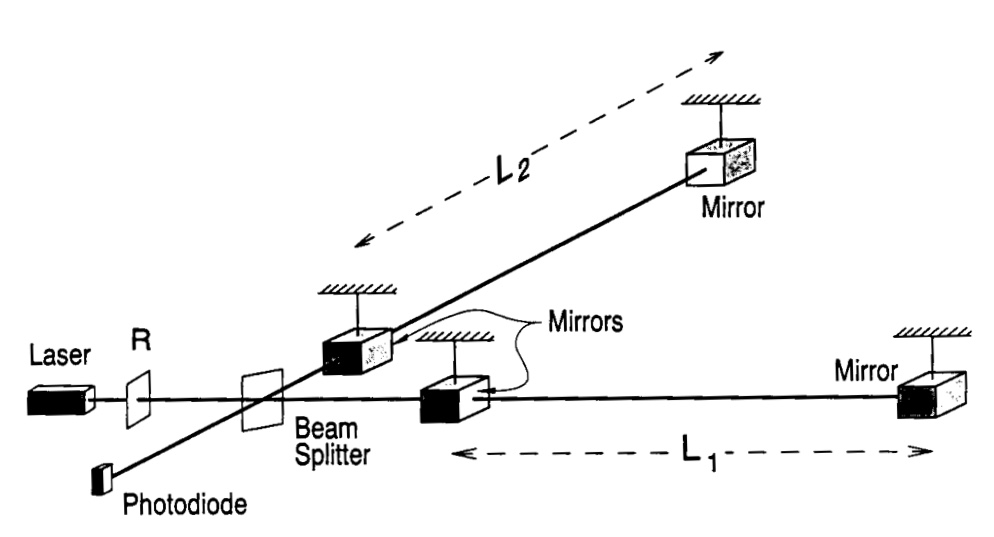
\includegraphics[width=0.9\textwidth]{effects_gw/interferometer}}
\caption{Schematic representation of a laser interferomenter gravitational wave detector (from REF).}
%A. Abramovici et. al. Science, 256:325, 1992: name in zoteroLIGO: The Laser Interferometer Gravitational-Wave Observatory
\label{interferometer}
\end{figure}
%%
%%
%%
%%



\subsection{From the geodesic deviation equation to the $+$ and $\times$ polarizations}
Since free-falling bodies obey to the geodesic equation(\ref{geodesic_eq}), in this section we study the physical effects of the two polarizations plus $+$ and times $\times$ of the gravitational waves through relative motions of geodesics.\\
The \textbf{geodesic deviation equation}  expresses the relative acceleration between two neighboring geodesics belonging to a one-parameter geodesics $\gamma_s (\tau)$:
\begin{equation}
\label{geudesic_deviation_eq}
\dfrac{D^2}{d \tau ^2} S^{\mu} = :R^{\mu} _{\nu \rho \sigma}: \, T^{\nu} T^{\rho} S^{\sigma}
\end{equation}
 where $S^{\mu} = \partial x^{\mu} / \partial s$ is the deviattion from the geodesic, $T^{\nu} = \partial x^{\mu} / \partial \tau$ is the tangent to the geodesic and the directional covariant derivative is 
\[
\dfrac{D}{d \tau} = \dv{x^{\mu}}{\tau} \, \nabla_{\mu}
\]
A non-zero acceleration of the deviation bewteen between neighbouring geodesics is a signature of spacetime curvature.
In fact, geodesic deviation cannot distinguish between a zero gravitational field and a uniform grabitational field. Only tidal gravitational fields give rise to an acceleration in the geodesic deviation. \\
Let us consider some nearby particles with four-velocities described by a single vector field $u^{\mu}$ and separation vector field $S^{\mu}$, the geodesic deviation equation(\ref{geudesic_deviation_eq}) becomes
\begin{equation}
\dfrac{D^2}{d \tau ^2} S^{\mu} = :R^{\mu} _{\nu \rho \sigma}: \, u^{\nu} u^{\rho} S^{\sigma}
\end{equation}
The four-velocity vector can be approximated with a unit vector in the time direction plus corrections of order $h^{\T} _{\mu \nu}$ and higher, however the Reimann curvature tensor is already first order. Therefore, we ignore the corrections of the four-velocity vector and we approximate $u^{\nu} =(1,0,0,0)$.\\
Since we have already calculated the Riemann curvature tensor in equation(\ref{reimann_tensor_TT}) taking into account the TT gauge conditions we recall the result
\bea
:R^\mu _{00 \sigma }: 
&=&
\dfrac{1}{2} \partial_0 \partial_0 :h^{\T \mu} _{\sigma}: 
\eea 
In the lowest order approximation the free-falling particles are slowly moving, then we have $\tau = x^{0} = t$, so the geodesic deviation equation becomes
\begin{equation}
\pdv[2]{}{t} S^{\mu} = \dfrac{1}{2} S^{\sigma} \pdv[2]{}{t} :h^{\T \mu} _{\sigma}:
\end{equation}
The above equation is a set of differential equations that can be rewritten using the two polarizations of the metric perturbation (equation(\ref{matrix_h_tt}))
\bea
\pdv[2]{}{t} S^{1} &=& \dfrac{1}{2} S^{1} \pdv[2]{}{t} h_{+} + \dfrac{1}{2} S^{2} \pdv[2]{}{t} h_{\times} \\
\pdv[2]{}{t} S^{2} &=& \dfrac{1}{2} S^{1} \pdv[2]{}{t} h_{\times} - \dfrac{1}{2} S^{2} \pdv[2]{}{t} h_{+}
\eea
These can be solved to yield, to lowest order,
\bea
S^{1} = S^{1}(t=0) \qty(1 + \dfrac{1}{2} h_{+})+ \dfrac{1}{2} h_{\times} S^{2}(t=0) \\
S^{2} = S^{2}(t=0) \qty(1 - \dfrac{1}{2} h_{+}) +  \dfrac{1}{2} h_{\times} S^{1}(t=0)
\eea
Let us study the effects of the two polarizations $h_{+}$ and $h_{\times}$ of a gravitational wave, which propagates through the center of a ring of free-falling test particles. 
So, let us use consider a plane wave travelling along the z axis, and let us place a ring of free-falling test particles on the x-y plane  with its center in $(0,0,0)$. 
The ring is initially parametrized by $(\cos \theta, \sin \theta)$ with $\theta \in (0,2\pi]$ and the separation vector $S^{\mu}$ measures the deformation of the ring from its center.\\
%%
%%
%%
%%
\begin{figure}
\centering
    \textbf{Time evolution of the $\mathlarger{\mathlarger{+}}$ polarization}\par\medskip
\makebox[\textwidth][c]{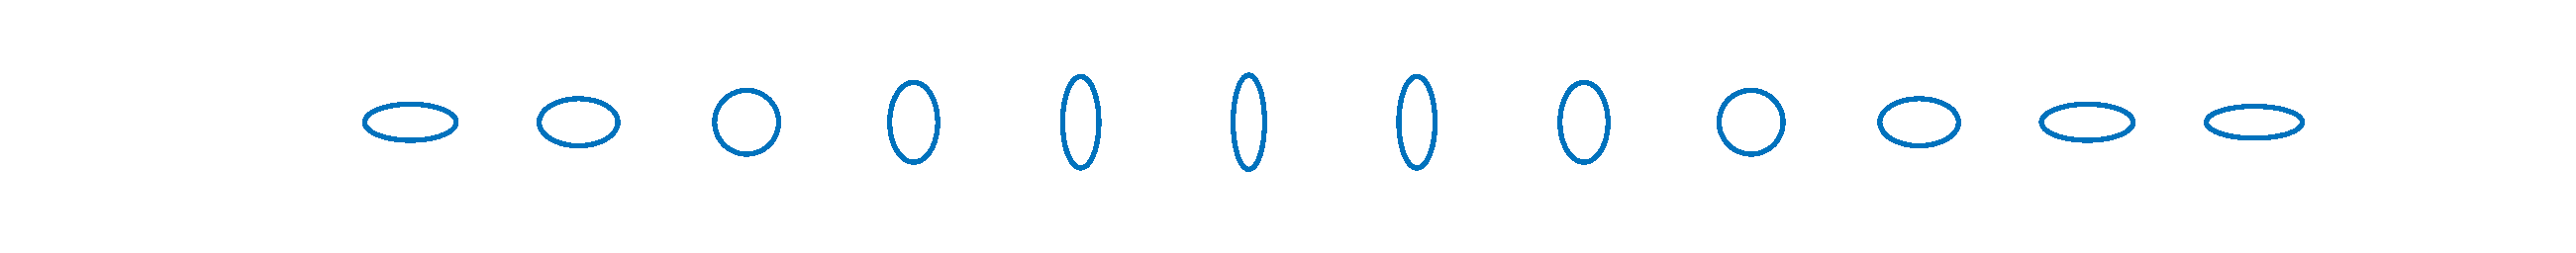
\includegraphics[width=1.3\textwidth]{effects_gw/plus_polarization.eps}}
\caption{Effect of the $h_+$ mode on a ring of free-falling test particles at $\omega t = n\pi/6 $ with $n=0,...,12$.}
\label{plus_polarization}
\end{figure}
%%
%%
%%
%%
\begin{figure}
\centering
\textbf{Time evolution of the $\mathlarger{\mathlarger{\times}}$ polarization.}\par\medskip
\makebox[\textwidth][c]{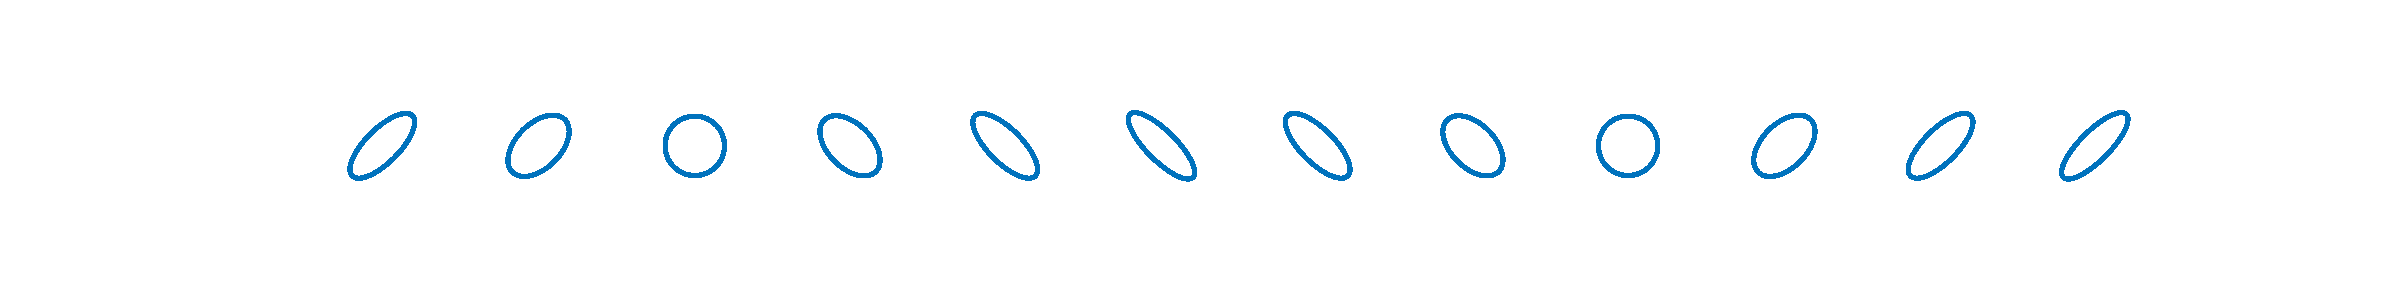
\includegraphics[width=1.3\textwidth]{effects_gw/times_polarization.eps}}
\caption{Effect of the $h_\times$ mode on a ring of free-falling test particles at $\omega t = n\pi/6 $ with $n=0,...,12$.}
\label{times_polarization}
\end{figure}
%%
%%
%%
%%
Beginning with the case $h_{\times} =0$ and $h_{+} \neq 0$, the solutions of the geodesic deviation equation are
\begin{eqnarray}
\label{s1_+}
S^{1}_{+} = \cos\theta \qty(1 + \dfrac{1}{2} A^{\T} _{11} \cos (\omega t)) \\
\label{s2_+}
S^{2}_{+} = \sin \theta \qty(1 - \dfrac{1}{2} A^{\T} _{11} \cos (\omega t))
\end{eqnarray}
where $h_{+} = A^{\T} _{11} \cos (\omega t)$ for a plane wave. 
The time evolution of the ring is shown in Figure(\ref{plus_polarization}).\\
When the plus polarized gravitational wave propagates through the ring, it increases the proper distance between the ring and its center along the x axis when the phase of the wave is close to $\omega t = 0, 2\pi$, meanwhile it squeezes the test particles along the y axis.
If the phase of the gravitational wave is close to $\omega t = \pi/2, 3\pi/2$ the ring is strecthed along the y axis and the test particles move inwards, therefore, the proper distance from the center of the ring is reduced.
As the wave passes, the test particles bounce back and forth in the shape of $+$ as shown in Figure(\ref{plus_cont}). \\
On the ohter hand, the case where $h_{\times} \neq 0$ and $h_{+} = 0$ yields the geodesic deviation solutions to be
\bea
S^{1}_{\times} =   \cos \theta + \dfrac{1}{2} \sin \theta A^{\T} _{12} \cos (\omega t) \\
S^{2}_{\times} = \sin \theta  +  \dfrac{1}{2}  \cos \theta A^{\T} _{12} \cos (\omega t)
\eea
where $h_{\times} = A^{\T} _{12} \cos (\omega t)$ for a plane wave. 
The relationship between these solutions and those for $h_{+} \neq 0$ can be easily found if we rotate the x and y axis through an angle of $ -\pi / 4 $, so that the new coordinate axis are
\bea
x' = \dfrac{1}{\sqrt{2}} (x-y)\\
y' = \dfrac{1}{\sqrt{2}} (x + y)\\
\eea
Then, the geodesic deviations $S_{+}$ of  equations (\ref{s1_+}) and (\ref{s2_+}) with $h_{+} \neq 0$ and $h_{\times} =0$ become
\bea
S' _{+}\, ^{1} = (S^{1}_{+} - S^{2}_{+})/\sqrt{2} = \cos \qty(\theta +\pi / 4 ) + \dfrac{1}{2} \sin \qty(\theta +\pi / 4 )  h_{+} 
\\
S' _{+}\, ^{2} = (S^{1}_{+} + S^{2}_{+})/\sqrt{2}  = \sin \qty(\theta +\pi / 4 )   +  \dfrac{1}{2}  \cos \qty(\theta +\pi / 4 )  h_{+}
\\
\eea
The above equations are similiar to those with $h_{+} = 0$ and $h_{\times} \neq 0$, in fact the deviations $S^{1} _{\times}$ and $S^{2} _\times$ are nothing but the plus polarization rotated of an angle $-\pi/4$. So, in this case ($h_{+} = 0$ and $h_{\times} \neq 0$) the circle of particles bounce back and forth in the shape of $\times$ as we can see from Figures (\ref{times_polarization}) and (\ref{times_cont}).
%%
%%
%%
%%
\begin{figure}
\centering
    \textbf{$\mathlarger{\mathlarger{+}}$ Polarization and $\mathlarger{\mathlarger{\times}}$ Polarization}\par\medskip
\centering
\subfloat[][$+$ polarized gravitational wave.]
   {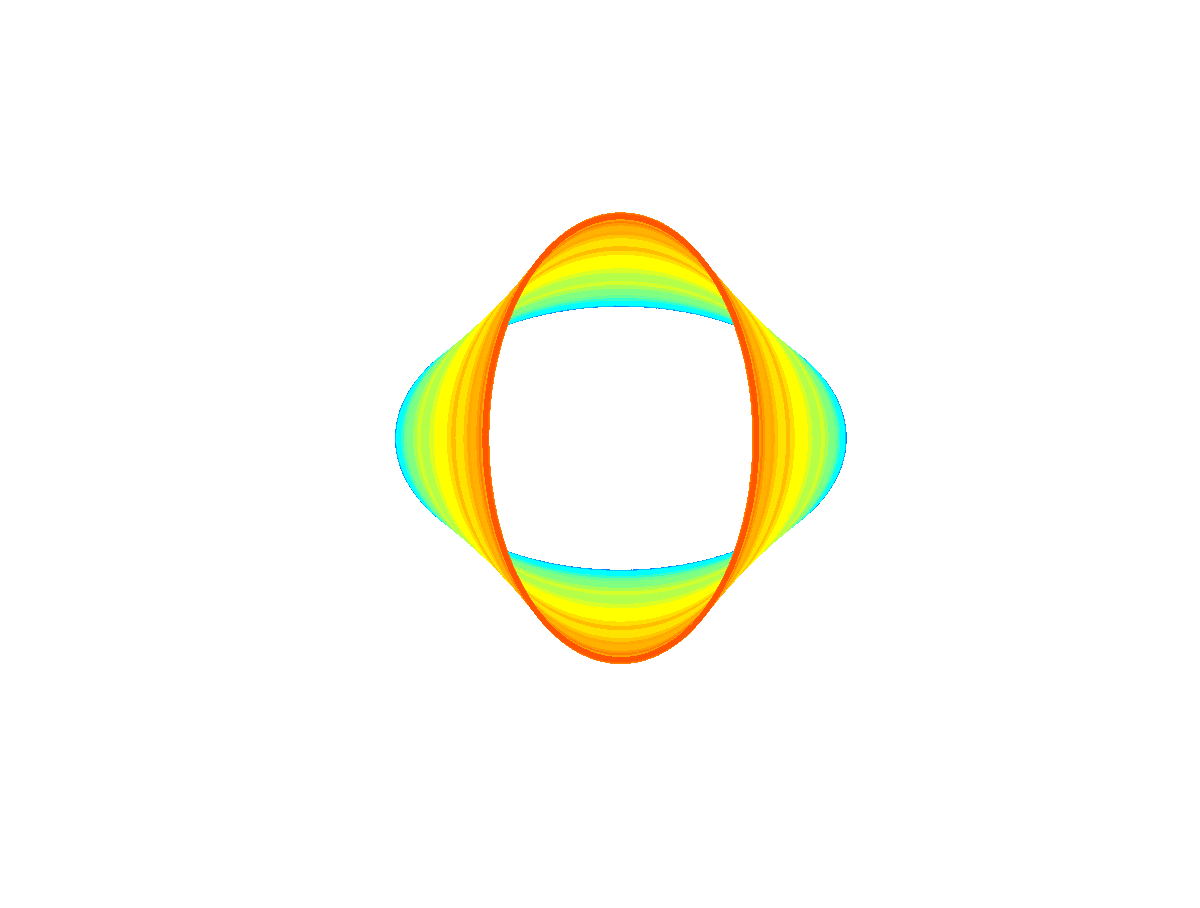
\includegraphics[width=.45\textwidth]{effects_gw/plus_pol_cont.eps}
   \label{plus_cont}} \quad
\subfloat[][$\times$ polarized gravitational wave.]
   {
\includegraphics[width=.45\textwidth]{effects_gw/times_pol_cont.eps}
   \label{times_cont}} \\
\caption{Spatial positions occupied by a ring of free-falling test particles disturbed by a gravitational wave.}
\label{plus_and_times}
\end{figure}
%%
%%
%%
%%
We could consider also right- and left-handed cricularly polarized modes by defining
\begin{eqnarray}
\label{r_polarized}
h_{R} = \dfrac{1}{\sqrt{2}} (h_{+} - i h_{\times})
\\
\label{l_polarized}
h_{L} = \dfrac{1}{\sqrt{2}} (h_{+} + i h_{\times})
\end{eqnarray}
The effect of a pure $h_R$ wave would be to rotate the particles in a right-handed sense and similiarly for the left-handed mode $h_{L}$. It is important to stress that the particles do not travel around the ring, they just move in little epicycles.
%%
%%
%%
%%
\begin{figure}
\centering
    \textbf{ Right- and Left-handed cricularly polarized modes}\par\medskip
\centering

\subfloat[][Right-handed polarized gravitational wave.]
   {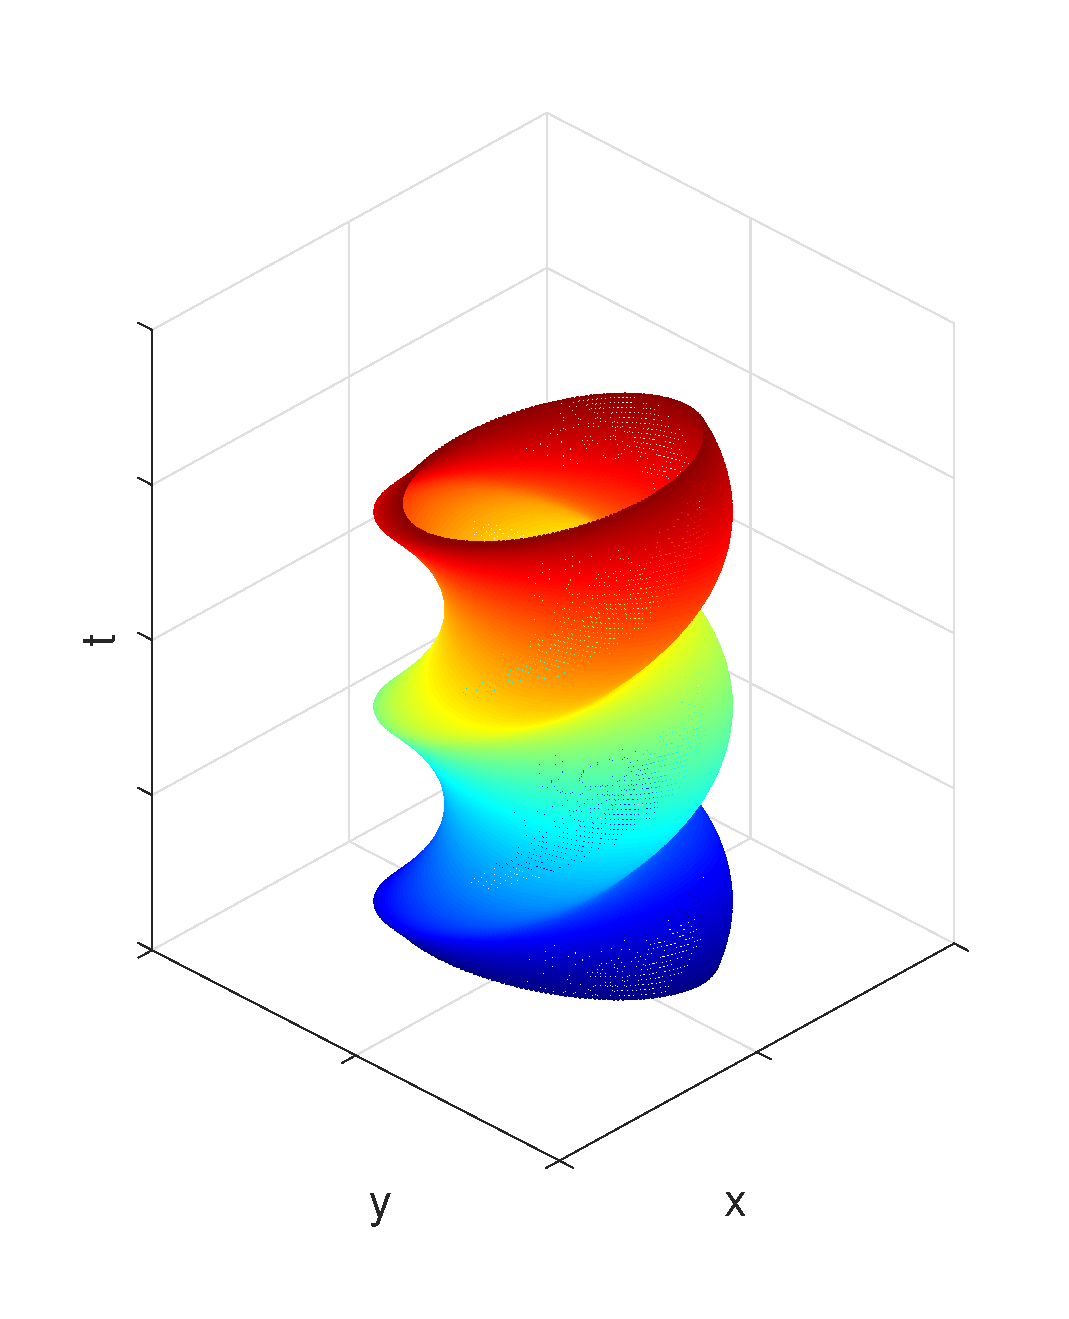
\includegraphics[width=.45\textwidth]{effects_gw/r_pol.eps}
   \label{plus_cont}} \quad
\subfloat[][Left-handed polarized gravitational wave.]
   {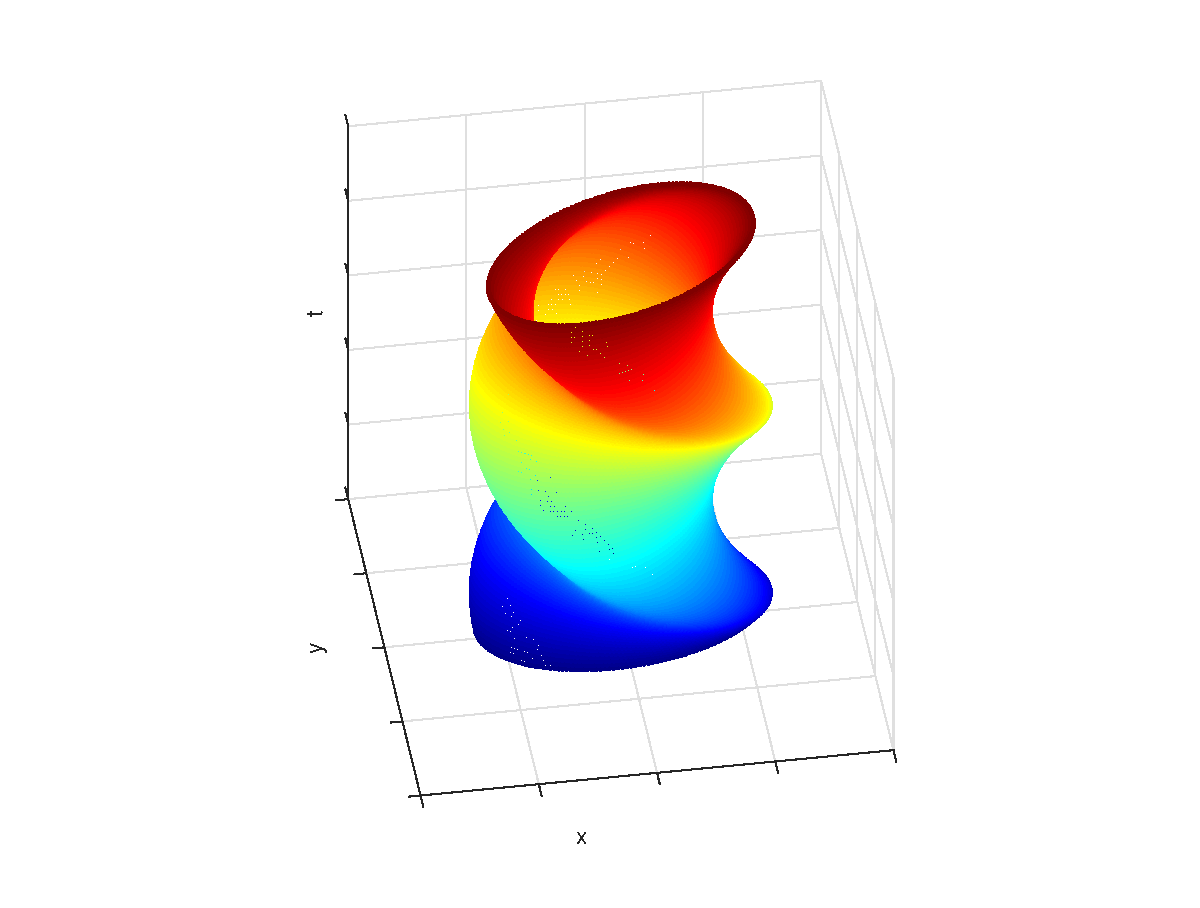
\includegraphics[width=.45\textwidth]{effects_gw/l_pol.eps}
   \label{times_cont}} \\
\caption{Time evoluition of a ring of free-falling test particles on the x-y plane.}
\label{plus_and_times}

\end{figure}




